% \documentclass{bookclass}

%% -------------------------------
%% |    ISSD Thesis Template       |
%% -------------------------------
%% Further additions by:
%%   Philipp Stroehle, IM, 2013 
%%   Jasper Feine, ISSD, 2018
%%   Merlin Knaeble, ISSD, 2020-2022 
%% firstname.lastname "at" kit.edu

%% Notes:
%% Language switch after \begin{document}

% Based on thesisclass.cls of Timo Rohrberg, 2009
% ----------------------------------------------------------------
% Thesis - Main document
% ----------------------------------------------------------------

\usepackage[english, german]{babel}
\usepackage{csquotes} % for citing more advanced

%% ---------------------------------
%% |      Additional packages      |
%% ---------------------------------
%% 

\usepackage{graphicx}
\DeclareGraphicsExtensions{.pdf,.png,.jpg}
\graphicspath{{./figures/},{./text/content/images/}} %Use curly braces for each path to add and don't forget trailing slash '/'
% \usepackage{epstopdf} %Nice to automatically convert eps figures to pdf format  (from inkscape, etc)
\usepackage[style=apa, backend=biber, natbib=true, hyperref=true, uniquelist=true, language=american]{biblatex}
\addbibresource{data/book/latex/non_peer_reviewed_literature.bib}
\addbibresource{non_peer_reviewed_literature.bib}
\usepackage{booktabs}

%% ---------------------------------
%% | Needed for the List of Abbreviations |
%% ---------------------------------
% create nomenclature
\usepackage{nomencl}
\renewcommand{\nomname}{List of Abbreviations}
\setlength{\nomlabelwidth}{.40\hsize}
\renewcommand{\nomlabel}[1]{#1 \dotfill}
\setlength{\nomitemsep}{-\parsep}
\makenomenclature
\usepackage[normalem]{ulem}
\newcommand{\markup}[1]{\uline{#1}}

\nomenclature{NaN}{Not a Number}
\nomenclature{\#}{number of}
\nomenclature{$\sigma(x)$}{Sigmoid function}
\nomenclature{$\rho(x)$}{Euclidian distance}
\nomenclature{$\chi(x)$}{indicator function}
\nomenclature{$\star$}{Cross-correlation operator}

% create glossary
\usepackage{glossaries}
\newglossaryentry{WebRTC}
{
    name=WebRTC,
    description={Web Real-Time Communication}
}

\newglossaryentry{i.i.d}
{
    name=i.i.d,
    description={independent and identically distributed}
}

\newglossaryentry{MS-COCO}
{
    name=MS-COCO,
    description={Microsoft Common Objects in Context is a dataset for common computer vision tasks: https://cocodataset.org/}
}

\newglossaryentry{YUV}
{
    name=YUV,
    description={Luminance(Y), chrominance component blue projection(U), chrominance component red projection(V) codification of an image}
}

\newglossaryentry{RGB}
{
    name=RGB,
    description={Red Green Blue codification of an image}
}

\newacronym{numberof}{\#}{number of}
\newacronym{sigmoidFunction}{$\sigma(x)$}{Sigmoid function}
\newacronym{euclidiandistance}{$\rho(x)$}{Euclidian distance}
\newacronym{chi}{$\chi(x)$}{indicator function}
\newacronym{star}{$\star$}{Cross-correlation operator}
\newacronym{nan}{NaN}{Not a Number}

\newacronym{sueq}{S-UEQ}{Short User Experience Questionnaire}
\newacronym{dram}{DRAM}{Dynamic Random Access Memory}
\newacronym{hsv}{HSV}{Hue Saturation Value}
\newacronym{csv}{CSV}{Comma-separated values}
\newacronym{cnn}{CNN}{Convolutional Neural Network}
\newacronym{rl}{RL}{Reinforcement Learning}
\newacronym{vr}{VR}{Virtual reality}
\newacronym{ueqs}{UEQ-S}{Short User Experience Questionnaire}
\newacronym{dtw}{DTW}{Dynamic time warping}
\newacronym{knn}{KNN}{k-nearest neighbors}
\newacronym{ciou}{CIoU}{Complete Intersection over Union}
\newacronym{mse}{MSE}{Mean Squared Error}
\newacronym{mscoco}{MSCOCO}{Microsoft Common Objects in Context}
\newacronym{bce}{BCE}{binary cross entropy}
\newacronym{silu}{SiLU}{sigmoid linear unit function}
\newacronym{relu}{ReLU}{rectified linear unit function}
\newacronym{csp}{CSP}{Cross stage partial}
\newacronym{spp}{SPP}{Spatial pyramid pooling}
\newacronym{pan}{PAN}{Path Aggregation Network}
\newacronym{fpn}{FPN}{Feature Pyramid Networks}
\newacronym{yolact}{YOLACT}{You Only Look At CoefficienTs}
\newacronym{uwp}{UWP}{Universal Windows Platform}
\newacronym{onnx}{onnx}{Open Neural Network Exchange}
\newacronym{ovr}{OvR}{One-vs-Rest}
\newacronym{cvf}{CVF}{Computer Vision Foundation}
\newacronym{tnr}{TNR}{True Negative Rate}
\newacronym{tpr}{TPR}{True Positive Rate}
\newacronym{fpr}{FPR}{False Positive Rate}
\newacronym{mts}{MTS}{multivariate time series}
\newacronym{fc}{FC}{Fully Connected}
\newacronym{mlp}{MLP}{Multi Layer Perceptron}
\newacronym{slr}{SLR}{Systematic Literature Review}
\newacronym{fov}{FOV}{Field of View}
\newacronym{ar}{AR}{Augmented Reality}
\newacronym{rq}{RQ}{Research Question}
\newacronym{tsc}{TSC}{Time Series Classification}
\newacronym{cv}{CV}{Computer Vision}
\newacronym{gpu}{GPU}{Graphics Processing Unit}
\newacronym{flops}{FLOPS}{Floating Point Operations per Second}
\newacronym{yolo}{YOLO}{You only look once}
\newacronym{ui}{UI}{User Interface}
\newacronym{fps}{FPS}{Frames per second}
\newacronym{ap}{AP}{Average Precision}
\newacronym{auc}{AUC}{Area Under Curve}
\newacronym{map}{mAP}{mean average precision}
\newacronym{iou}{IOU}{Intersection over Union}
\newacronym{ml}{ML}{Machine learning}
\newacronym{roc}{ROC}{Receiver operating characteristic}
\newacronym{mrtk}{MRTK}{Mixed Reality Toolkit}
\newacronym{svm}{SVM}{Support Vector Machines}
\newacronym{nn}{NN}{Neural Nets}
\newacronym{crisp}{CRISP-DM}{Cross-industry standard process for data mining}
\newacronym{mr}{MR}{Mixed Reality}
\newacronym{lr}{LR}{Learning Rate}
\newacronym{sgd}{SGD}{Stochastic gradient descent}
\newacronym{tp}{TP}{True Positive}
\newacronym{tn}{TN}{True Negative}
\newacronym{fp}{FP}{False Positive}
\newacronym{fn}{FN}{False Negative}
\newacronym{pr}{PR}{Precision-Recall}

\makeglossaries

% \usepackage{lipsum} % if you use some additional packages
% \titleformat{\chapter}[hang]{\huge\bfseries}{\thechapter.}{2pc}{}

%% ---------------------------------
%% | Information about the book    |
%% ---------------------------------

\newcommand{\mytitle}{Computer Graphics}
\newcommand{\mytitleger}{Introduction into the world of rendering}

\newcommand{\reviewerone}{Max Mustermann}
\newcommand{\reviewertwo}{Johannes Heinle}
\newcommand{\submissiontime}{22.05.2023}

\newcommand{\myname}{Jonas Heinle}
%% -------------------------------
%% |  Information for PDF file   |
%% -------------------------------
\hypersetup{
	pdfauthor={\myname},
	pdftitle={\mytitle},
	pdfsubject={\mytitle},
	pdfkeywords={\mytitle}
}

%% --------------------------------
%% | Settings for word separation |
%% --------------------------------
% Describe separation hints here:
\hyphenation{
	opos-sum
	he-lio-trope
}

%% --------------------------------
%% | Include C-style pseudo code |
%% --------------------------------
\lstset{
  basicstyle=\footnotesize,        % the size of the fonts that are used for the code
  breakatwhitespace=false,         % sets if automatic breaks should only happen at whitespace
  captionpos=b,                    % sets the caption-position to bottom
  commentstyle=\color{mygreen},    % comment style
  deletekeywords={...},            % if you want to delete keywords from the given language
  escapeinside={\%*}{*)},          % if you want to add LaTeX within your code
  extendedchars=true,              % lets you use non-ASCII characters; for 8-bits encodings only, does not work with UTF-8
  keepspaces=true,                 % keeps spaces in text, useful for keeping indentation of code (possibly needs columns=flexible)
  keywordstyle=\color{blue},       % keyword style
  language=C,                      % the language of the code
  morekeywords={*,...},            % if you want to add more keywords to the set
  %numbers=left,                   % where to put the line-numbers; possible values are (none, left, right)
  numbersep=7pt,                   % how far the line-numbers are from the code
  numberstyle=\tiny\color{mygray}, % the style that is used for the line-numbers
  rulecolor=\color{black},         % if not set, the frame-color may be changed on line-breaks within not-black text (e.g. comments (green here))
  showspaces=false,                % show spaces everywhere adding particular underscores; it overrides 'showstringspaces'
  showstringspaces=false,          % underline spaces within strings only
  showtabs=false,                  % show tabs within strings adding particular underscores
  stepnumber=1,                    % the step between two line-numbers. If it's 1, each line will be numbered
  stringstyle=\color{mymauve},     % string literal style
  tabsize=4,	                     % sets default tabsize to 2 spaces
}

%% ------------------------
%% |    Including files   |
%% ------------------------
% Only files listed here will be included!
% Userful command for partially translating the document (for bug-fixing e.g.)
% \includeonly{
% titlepage,
% text/dedication,
% text/acknowledgment,
% text/abstract,
% text/content,  %feel free to introduce additional files for structuring your thesis
% text/appendix
% }

%%%%%%%%%%%%%%%%%%%%%%%%%%%%%%%%%
%% Here, main documents begins %%
%%%%%%%%%%%%%%%%%%%%%%%%%%%%%%%%%
% \begin{document}

% \frontmatter
% %% titlepage.tex
%%

% coordinates for the bg shape on the titlepage
\newcommand{\diameter}{20}
\newcommand{\xone}{-15}
\newcommand{\xtwo}{160}
\newcommand{\yone}{15}
\newcommand{\ytwo}{-253}

\begin{titlepage}
% bg shape
\begin{tikzpicture}[overlay]
\draw[color=gray]  
 		 (\xone mm, \yone mm)
  -- (\xtwo mm, \yone mm)
 arc (90:0:\diameter pt) 
  -- (\xtwo mm + \diameter pt , \ytwo mm) 
	-- (\xone mm + \diameter pt , \ytwo mm)
 arc (270:180:\diameter pt)
	-- (\xone mm, \yone mm);
\end{tikzpicture}
	\begin{center}
		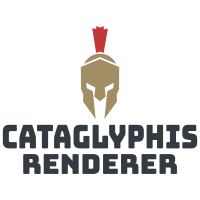
\includegraphics[width=.3\textwidth]{logos/Engine_logo.png} % KITLogo_EN_RGB.pdf
	\end{center}
	\changefont{ppl}{m}{n}	% helvetica	(phv), % IM Style: palatino (ppl) 
	\vspace*{0.5cm}
	\begin{center}
		\Huge{\mytitle}\\
		\rule{0.05\textwidth}{0.5pt}\\
		\Large{\mytitleger}\\
		\vspace*{1cm}
		\huge{\myname}\\
            \github{Kataglyphis}%\newline
		\vspace*{1cm}
	\end{center}
	%\vspace*{1cm}
\Large{
\begin{center}
\begin{tabular}[ht]{l c l}
  Reviewer: & \hfill  & \reviewerone\\
  Second Reviewer: & \hfill  & \reviewertwo\\
\end{tabular}
\end{center}
}

\vspace{1.cm}
\begin{center}
\large{\submissiontime}
% \iflanguage{english}{Duration:}{Bearbeitungszeit:} \timestart \hspace*{0.25cm}
% -- \hspace*{0.25cm} 
% \timeend}
\end{center}


\begin{textblock}{10}[0,0](5,16.8)
\large{ 
	Jonas Heinle
}
\end{textblock}

\begin{textblock}{10}[0,0](12,16.8)
\large{
	\textbf{\url{www.jotrockenmitlocken.de}} 
}
\end{textblock}

\end{titlepage}
% \pagenumbering{roman}
% \include{text/dedication}
% \include{text/acknowledgment.tex}
% \include{text/abstract}

% % ISSD Style: No additional blank page
% % \blankpage


% %% -------------------
% %% |   Directories   |
% %% -------------------
% \tableofcontents

% % ISSD Style: No additional blank page
% % \blankpaage

% % You may elect not to include a list of figures, list of tables and list of abbreviations, if the work is a seminar thesis (comment out the following)
% \listoffigures \addcontentsline{toc}{chapter}{List of Figures} 
% \listoftables  \addcontentsline{toc}{chapter}{List of Tables} 
% % \printnomenclature   \addcontentsline{toc}{chapter}{List of Abbreviations} 
% %\printglossaries  \addcontentsline{toc}{chapter}{List of Abbreviations}
% \printglossary[title=List of Abbreviations]

% %% -----------------
% %% |   Main part   |
% %% -----------------
% \mainmatter
% \pagenumbering{arabic}
% \include{text/content}


% \backmatter
% \pagenumbering{Roman}


% %% --------------------
% %% |   Bibliography   |
% %% --------------------

% % src: https://tex.stackexchange.com/questions/112874/sectioning-bibliography-by-type-with-multiple-types-per-section
% \defbibfilter{papers}{
%   type=article or
%   type=inproceedings or 
%   type=incollection or
%   type=book
% }

% \phantomsection
% \addcontentsline{toc}{chapter}{\bibname}
% \printbibliography[filter=papers]

% %% ----------------
% %% |   Appendix   |
% %% ----------------

% \input{text/appendix}

% \include{text/affidavit}
% \include{text/prototype_agreement}
% \end{document}